\documentclass[a4paper]{article}

\usepackage[brazilian]{babel}
\usepackage[utf8x]{inputenc}
\usepackage[T1]{fontenc}

\usepackage{float}

\usepackage{listings}
\usepackage{pythonhighlight}

%% Useful packages
\usepackage{amsmath}
\usepackage{graphicx}
\usepackage[colorinlistoftodos]{todonotes}
\usepackage[colorlinks=true, allcolors=blue]{hyperref}

\usepackage{mathrsfs}
\usepackage{amssymb}



%opening
\title{Relatório do Projeto 2}
\author{Daniel Moreira Cestari - 5746193}

\begin{document}

\maketitle

\section{Introdução}

O objetivo do Projeto 2 é o desenvolvimento de uma triangulação \textit{Delaunay} 2D. 

A definição de uma triangulação \textit{Delaunay} é uma triangulação de pontos tal que nenhum ponto do conjunto inicialmente fornecido está dentro do circuncirculo de qualquer triângulo da triangulação. Essa propriedade de nenhum ponto externo aos triângulos estar dentro do circuncirculo, garante que o mínimo ângulo dos triângulos será maximizado. É provado que dado um conjunto de pontos no espaço Euclidiano, a triangulação \textit{Delaunay} desses pontos é única, isso permite que a implementação deste trabalho possa ser testada utilizando outra biblioteca que já a implementa.

A entrada do algoritmo é um conjunto de pontos, e como saída o programa retorna na representação de uma \textit{Corner table} a triangulação \textit{Delaunay}  dos pontos passados.  O algoritmo para a triangulação empregado foi o algoritmo de inserção de pontos incrementalmente com \textit{flip} de arestas.

A estrutura de dados \textit{Corner table} foi implementada em atividade passadas da disciplina, mas até então possuía apenas operações de conjunta básica sobre os triângulos representados pela estrutura. Essas operações eram: fecho, estrela, anel, e \textit{link}. Para este trabalho foi necessário a inclusão de mais operações, como adição, remoção de triângulos, adição de vértices, busca de triângulos que compartilhem aresta, encontrar o triângulo que um dado ponto se encontra, coordenadas baricêntricas de um dado ponto, teste de orientação de pontos, teste do incirculo e \textit{flip} de arestas.



\section{Implementação}

Nesta seção é apresentada a implementação do código.

Abaixo é apresentado o esquema geral da implementação:
\begin{itemize}
	\item Determinação de um triângulo contendo os dados fornecidos (triângulo externo);
	
	\item Inserção incremental dos pontos fornecidos;
	\begin{itemize}
			\item Correção dos triângulos pelo teste do incírculo e \textit{flip} de arestas;
	\end{itemize}
	
	\item Remoção de todos os triângulos com vértices do triângulo externo;
	
	\item Limpeza da estrutura de dados de objetos eliminados.
	
\end{itemize}

Abaixo é exibida a função que calcula a triangulação:
%%%%%%%%%%%%%%%%%%%%
% def delaunay_triangulation
\inputpython{project2.py}{12}{182}
%%%%%%%%%%%%%%%%%%%%



A seguir, cada etapa será descrita com mais detalhes.

Na \textit{docstring} de cada método é apresentada uma descrição geral da função e de cada parâmetro.

\subsection{Determinação do triângulo externo}

Nesta etapa os pontos são centrado, é tomada a distância do ponto mais distante da origem como o raio de um círculo que engloba todos os pontos. Esse raio é definido como a coordenada $y$ do primeiro vértice do triângulo, a coordenada $x$ é definida como $0$. Para encontrar os outros dois pontos é feita uma rotação de $\frac{-2\pi}{3} rad$ do ponto inicial duas vezes. Por fim, aos pontos encontrados são levados para a localização inicial dos dados.

A seguir é mostrado a função que calcula os vértices do triângulo externo.
%%%%%%%%%%%%%%%%%%%%
% def outer_triangle
\inputpython{project2.py}{224}{254}
%%%%%%%%%%%%%%%%%%%%


Próximas funções

% find_triangles
% triangle_share_edge
% remove_triangle
% add_triangle
% legalize
% _clean_table





\subsection{Particionamento do domínio e determinação dos bordos}

A função \textit{partitionate\_domain} chama as funções que realizam o particionamento e determinação dos bordos, \textit{heuristic\_1} e \textit{heuristic\_2}. Para a reutilização do código que resolve a equação de \textit{Laplace} cada partição é salva em arquivo, e essa função que salva cada partição em arquivo.
Abaixo é mostrada a função.

%%%%%%%%%%%%%%%%%%%%
% def partitionate_domain
%\inputpython{project1.py}{438}{484}
%%%%%%%%%%%%%%%%%%%%

A diferença entre as duas heurísticas está na divisão feita sobre as partições que contém o círculo.

A primeira heurística (função \textit{heuristic\_1}), na partição do círculo, define o bordo de cima como a parte de cima do domínio mais a reta vertical até chegar ao círculo, e o mesmo princípio para o bordo de baixo, seguindo o sentido da esquerda para a direita. Os bordos da esquerda e direita são definidos pela reta vertical e pela curva, dependendo se a partição está a direita ou a esquerda da curva, e seguindo o sentido de baixo para cima.
As figuras \ref{fig:heuristic1_top1} e \ref{fig:heuristic1_top2} mostram as malhas geradas pela heurística 1 nas partições do círculo. As cores definem os bordos, azul bordo de cima, laranja bordo de baixo, verde bordo da esquerda, e vermelho bordo da direita.

Após a apresentação do trabalho foi incorporado o refinamento dos bordos na heurística 1, e foram removidas as singularidades, quadriláteros com um dos lados de comprimento zero.



%%%%%%%%%%%%%%%%%%%%
% def heuristic_1
%\inputpython{project1.py}{78}{256}
%%%%%%%%%%%%%%%%%%%%





A heurística 2 difere da 1, na sua definição dos bordos sobre a partição da curva. Neste caso, a divisão é feita seguindo o lado, se lado em questão está a esquerda então é o bordo esquerdo, se está a direita é o bordo direito, se está acima é o de cima e se está abaixo o de baixo. Esta heurística não apresenta refinamento nos bordos.
As figuras \ref{fig:heuristic2_top1} e \ref{fig:heuristic2_top2} mostram malhas geradas utilizando a heurística 2, as cores têm o mesmo significado que o relatado na heurística 1.



%%%%%%%%%%%%%%%%%%%%
% def heuristic_2
%\inputpython{project1.py}{260}{433}
%%%%%%%%%%%%%%%%%%%%


\subsection{Geração da malha}

A função que gera a malha chama as funções que criam o domínio e o particionam, e depois resolve a equação de \textit{Laplace} em cada partição individualmente. Após a malha de cada partição ser gerada, elas são unidas em duas malhas e então o refinamento é realizado resolvendo a equação de \textit{Poisson} nas duas malhas finais. Mesmo que um refinamento utilizando as funções de controle não seja realizado, como a equação de \textit{Laplace} é utilizada novamente com as malhas unidas, é feita uma suavização nos pontos de união das malhas.

Essa é a principal função que chama todas as outras necessárias, e por isso é cheia de parâmetros. Todos descritos na \textit{docstring}, basicamente juntou todos os parâmetros das funções anteriores mais os parâmetros relativos ao refinamento da malha.

Abaixo é apresentada a função \textit{generate\_grid}.

%%%%%%%%%%%%%%%%%%%%
% def generate_grid
%\inputpython{project1.py}{489}{729}
%%%%%%%%%%%%%%%%%%%%

O arquivo \textit{VTK} final é o resultado da união das duas malhas finais refinadas. Foi preciso modificar o código original que gerava o \textit{VTK} para receber uma lista de malhas e quando salvar em disco, produzir apenas um arquivo. Foi tomado o cuidado para vértices posicionados na mesma posição não aparecerem repetidos, ou seja, as malhas são realmente unidas.


\section{Resultados}


Nesta seção serão apresentados os resultados obtidos com a implementação descrita anteriormente. Primeiro serão mostradas as malhas para a heurística 1 variando o número de pontos na malha, em seguida será feito o mesmo para a heurística 2.
A configuração do domínio e da curva será a mesma para ambas as heurísticas.

Após a apresentação do trabalho foram apontados algumas correções, agora incorporadas, mas devido às modificações o exemplo utilizando o aerofólio ficou ruim e foi removido deste relatório.

Todos os arquivos VTK gerados foram anexados.

\subsection{Heurística 1}

Código para gerar uma malha com 52 pontos nos bordos esquerdo e direito. Curva gerada com 52 pontos, centrada na origem, domínio com comprimento 10, altura 8, e comprimento 3 à direita da curva. O domínio é divido em 4 partes, e o refinamento é deixado apenas nos bordos e a equação de \textit{Laplace} propaga esse refinamento para o interior do domínio.


\begin{verbatim}
import imp
import numpy as np
from matplotlib import pyplot as plt
import project1 as pjt

imp.reload(pjt);  
grid = pjt.generate_grid(resolution=52, left_border=3, domain_length=10, 
domain_height=4, curve_params={"radius":1}, equation=pjt.circle, 
filename_curve="", heuristic=pjt.heuristic_1, k=3, filename_borders="circle_h1_50pts", plot=True)
\end{verbatim}

Abaixo o código agora utilizando 100 pontos.
\begin{verbatim}
import imp
import numpy as np
from matplotlib import pyplot as plt
import project1 as pjt

imp.reload(pjt);  
grid = pjt.generate_grid(resolution=100, left_border=3, domain_length=10, 
domain_height=4, curve_params={"radius":1}, equation=pjt.circle, 
filename_curve="", heuristic=pjt.heuristic_1, k=3, filename_borders="circle_h1_100pts", plot=True)
\end{verbatim}


%\begin{figure}[H]
%	\centering
%	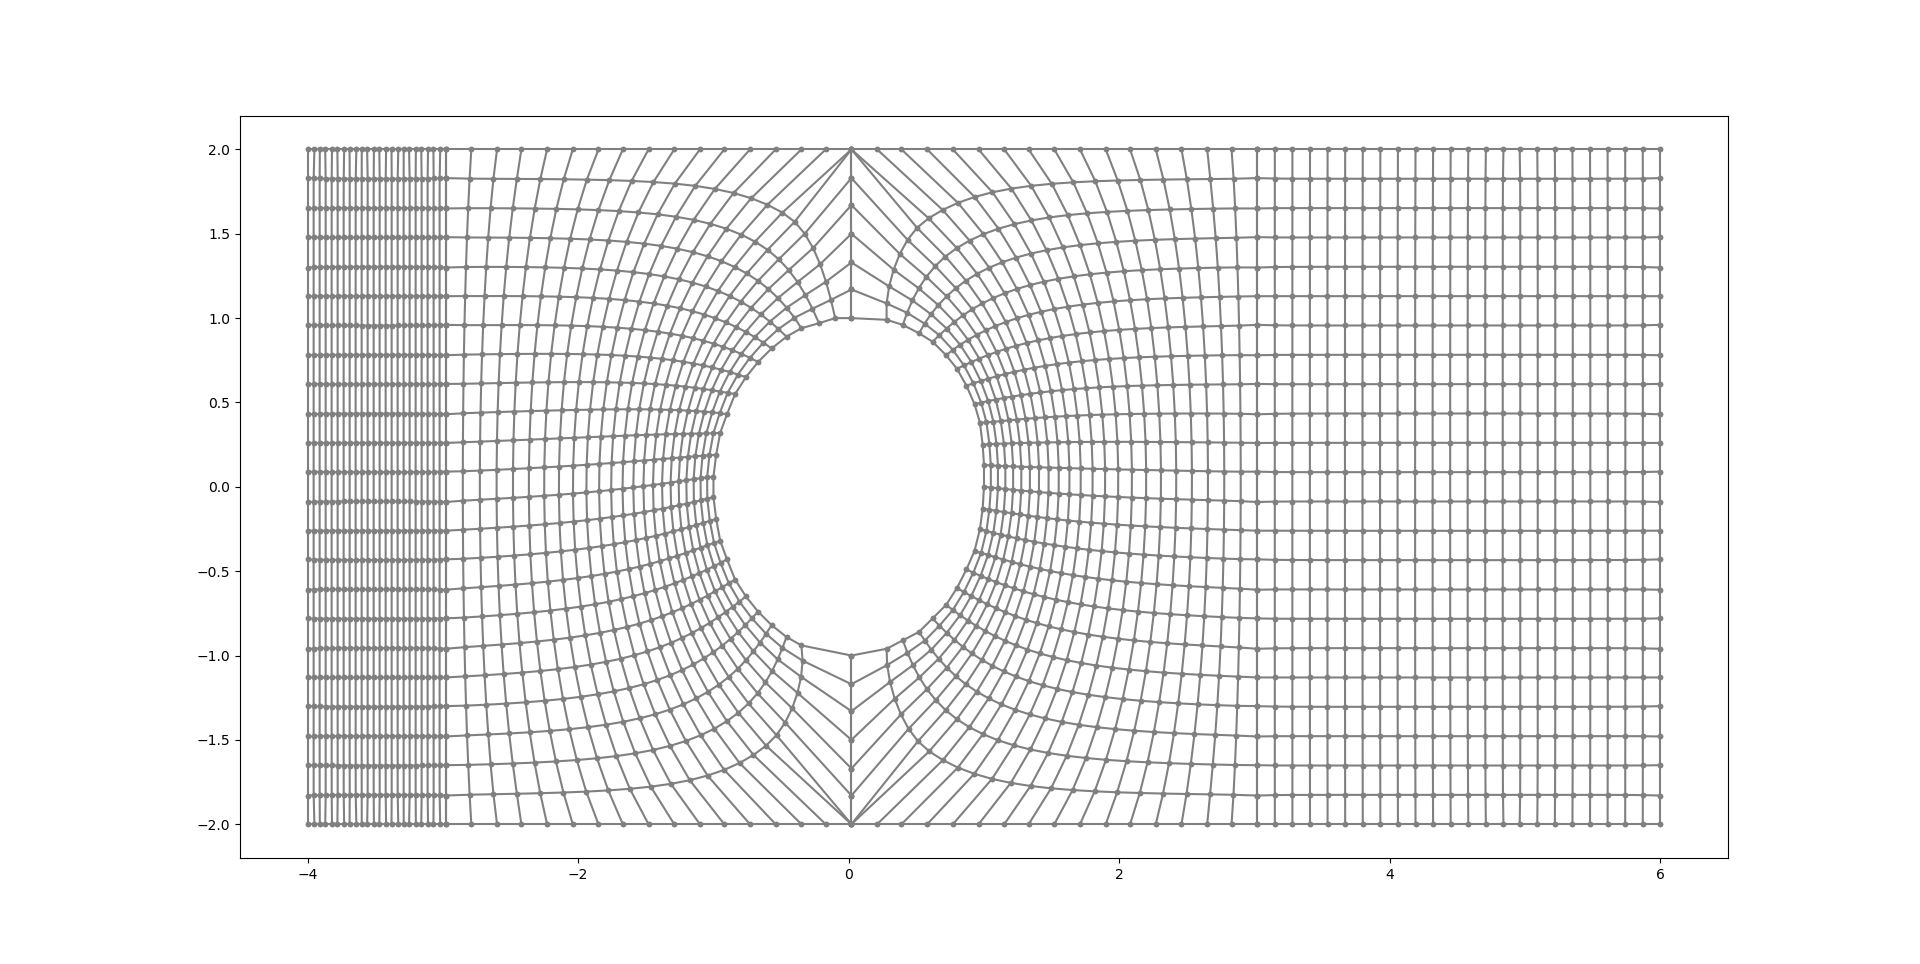
\includegraphics[width=1.0\textwidth]{heuristica_1_50pts.png}
%	\label{fig:heuristic1_50pts} 
%	\caption[caption]{Malha gerada pela heurística 1 com 50 pontos.}
%\end{figure}
%
%\begin{figure}[H]
%	\centering
%	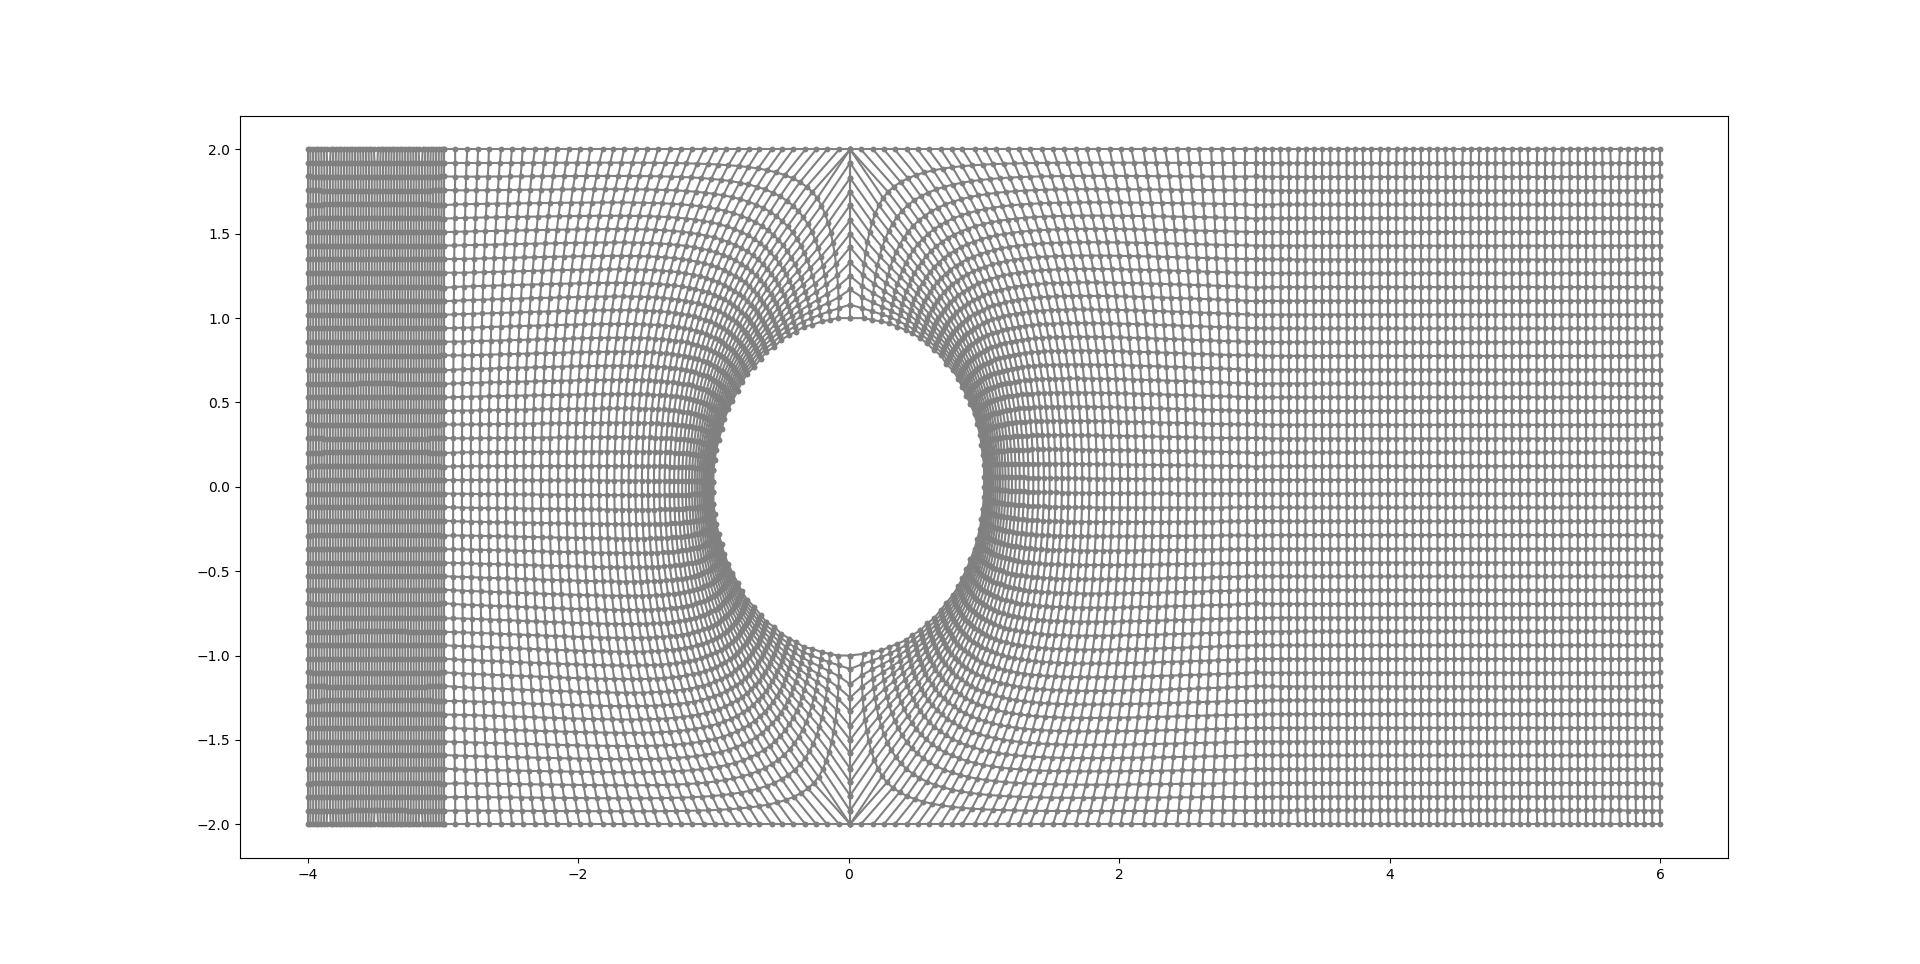
\includegraphics[width=1.0\textwidth]{heuristica_1_100pts.png}
%	\label{fig:heuristic1_100pts} 
%	\caption[caption]{Malha gerada pela heurística 1 com 100 pontos.}
%\end{figure}



\begin{figure}[H]
	\centering
	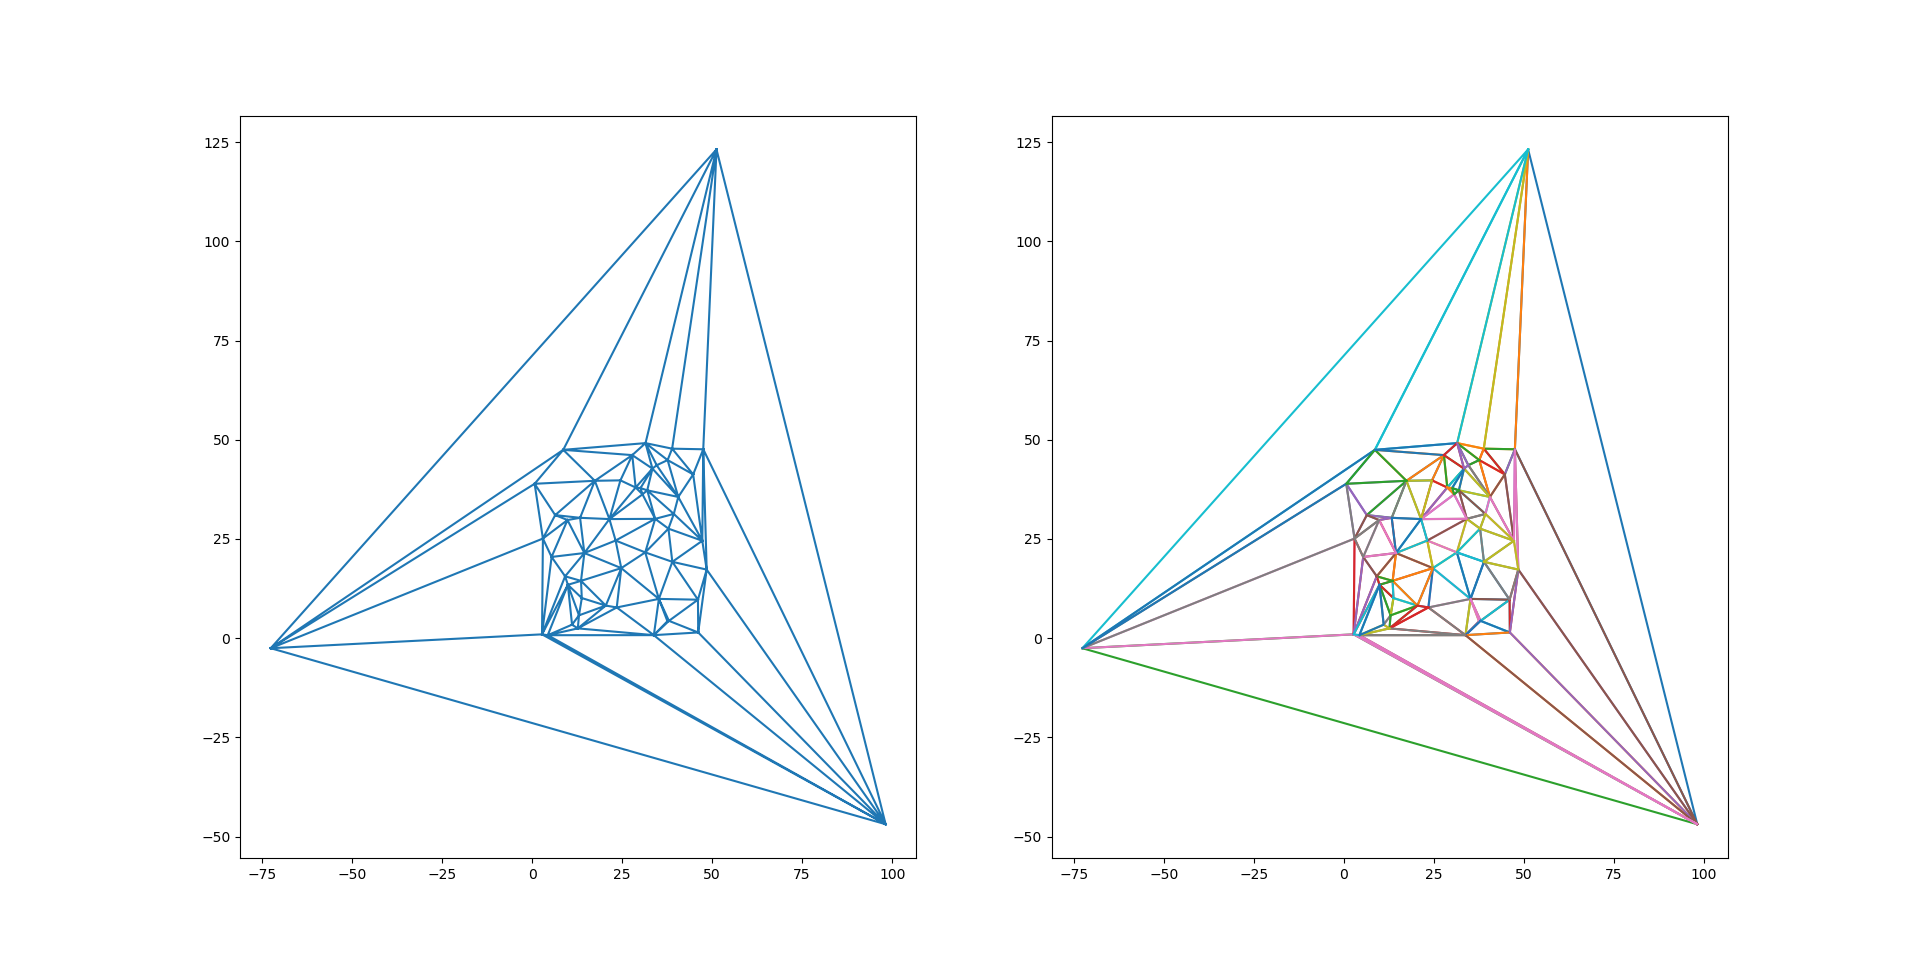
\includegraphics[width=1.0\textwidth]{./imgs/ex1_not_convex_outer.png}
	\label{fig:heuristic1_50pts_refined} 
	\caption[caption]{}
\end{figure}

\begin{figure}[H]
	\centering
	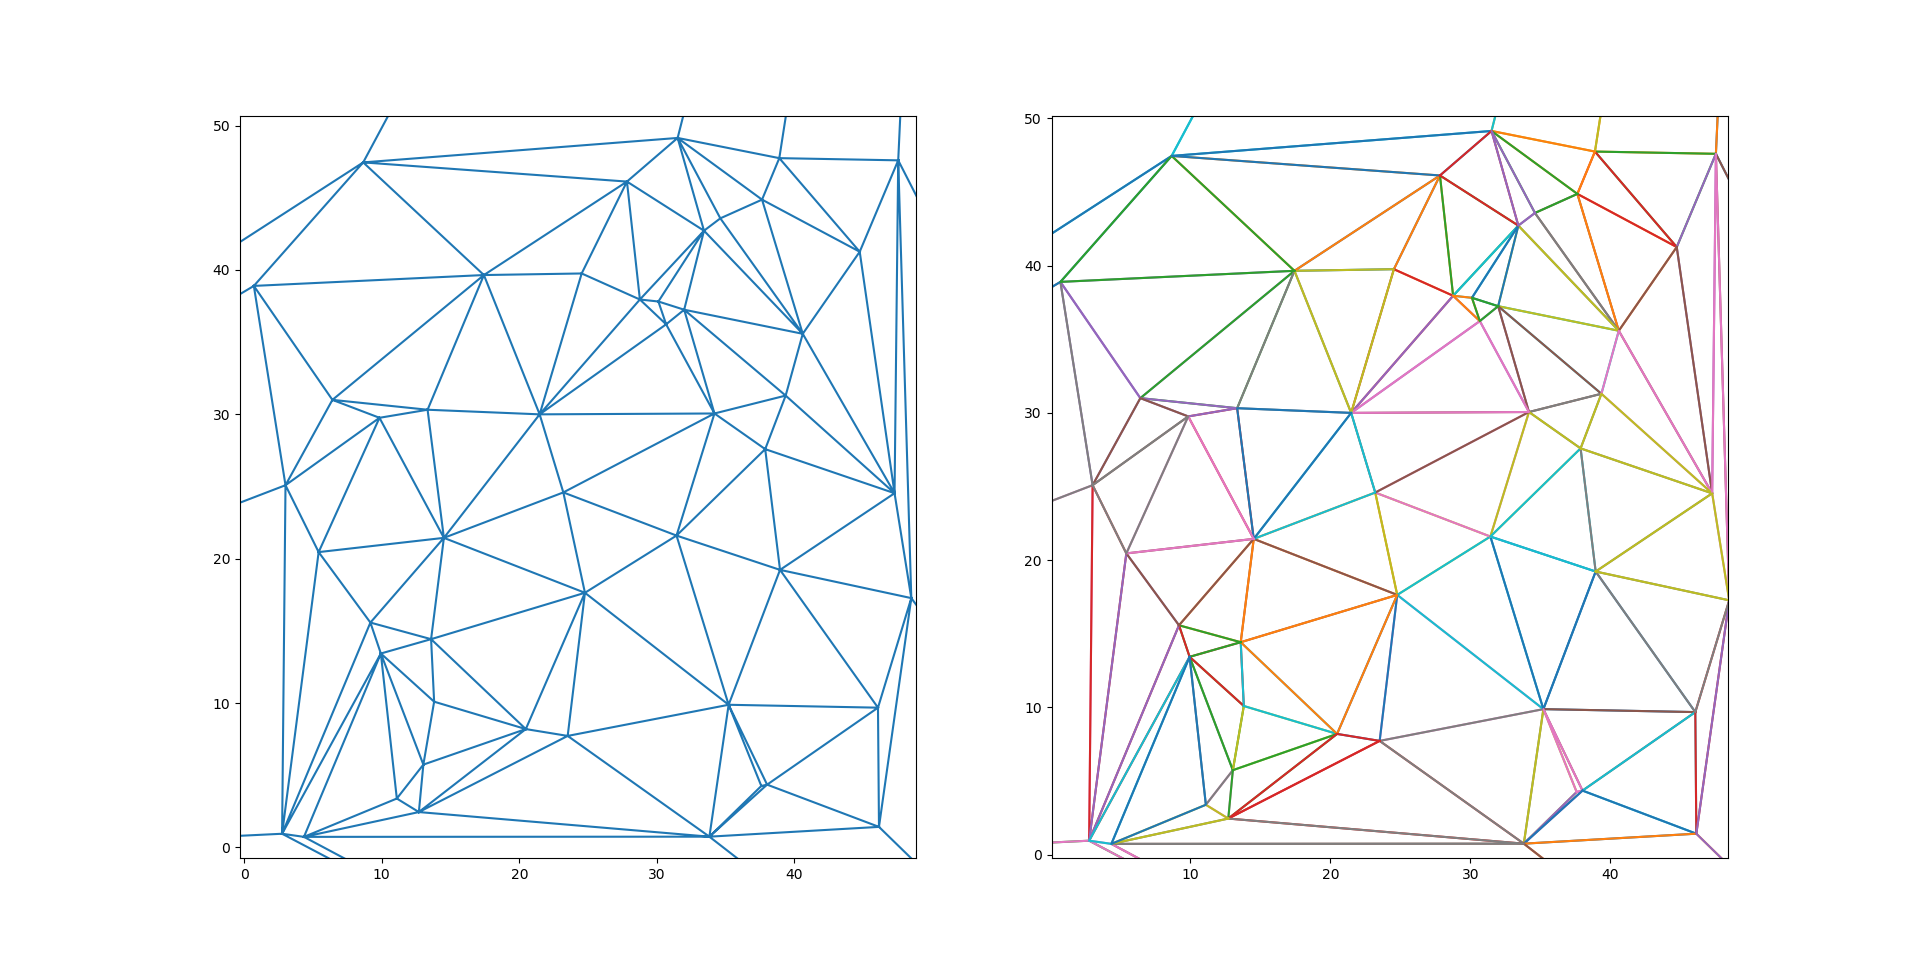
\includegraphics[width=1.0\textwidth]{./imgs/ex1_not_convex_outer_zoom.png}
	\label{fig:heuristic1_100pts_refined} 
	\caption[caption]{}
\end{figure}



\begin{figure}[H]
	\centering
	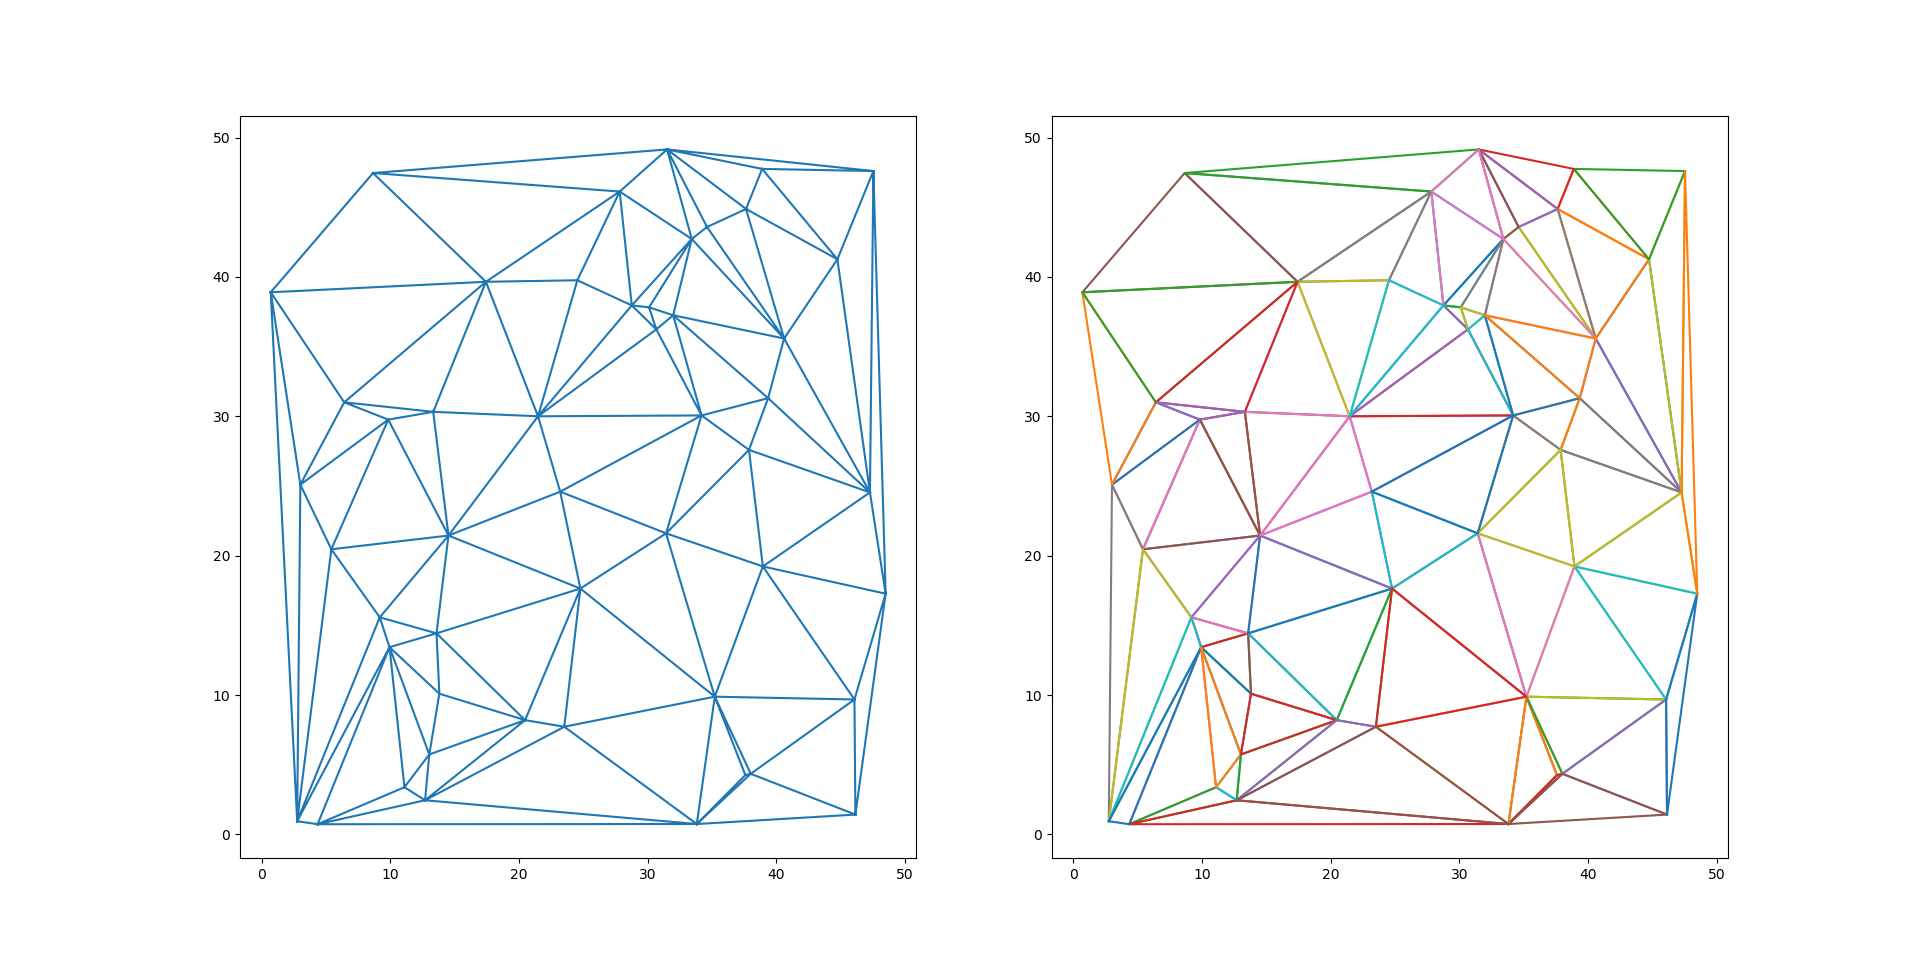
\includegraphics[width=1.0\textwidth]{./imgs/ex1_not_convex.png}
	\label{fig:heuristic1_100pts_refined} 
	\caption[caption]{}
\end{figure}





%
%\subsection{Aerofólio}
%
%Código para gerar uma malha para a curva \textit{naca012}, a resolução da malha é determinada pela quantidade de pontos na curva. O domínio com comprimento 4, altura 6, e comprimento 1 à direita da curva. O domínio é divido em 4 partes, e o refinamento é feito ao redor da curva e após a curva no centro do domínio em relação à \textit{y}, ou $\eta$.
%
%
%Código utilizando a heurística 1.
%\begin{verbatim}
%imp.reload(pjt);  
%grid = pjt.generate_grid(filename_curve="naca012.txt", 
%left_border=1, domain_length=4, domain_height=3,
%heuristic=pjt.heuristic_1, k=3, filename_borders="naca012_h1", 
%xis_rf0=[1], xis_rf1=[0], etas_rf1=[0.419], a_xis0=[5], 
%a_xis1=[2.5], c_xis0=[5], c_xis1=[5], a_etas1=[5], c_etas1=[15])
%\end{verbatim}
%
%Código utilizando a heurística 2.
%\begin{verbatim}
%imp.reload(pjt);  
%grid = pjt.generate_grid(filename_curve="naca012.txt", 
%left_border=1, domain_length=4, domain_height=3,
%heuristic=pjt.heuristic_2, k=3, filename_borders="naca_h2", 
%xis_rf0=[1], xis_rf1=[0], etas_rf1=[0.419], a_xis0=[5], 
%a_xis1=[2.5], c_xis0=[5], c_xis1=[5], a_etas1=[5], c_etas1=[15])
%\end{verbatim}
%
%
%\begin{figure}[H]
%	\centering
%	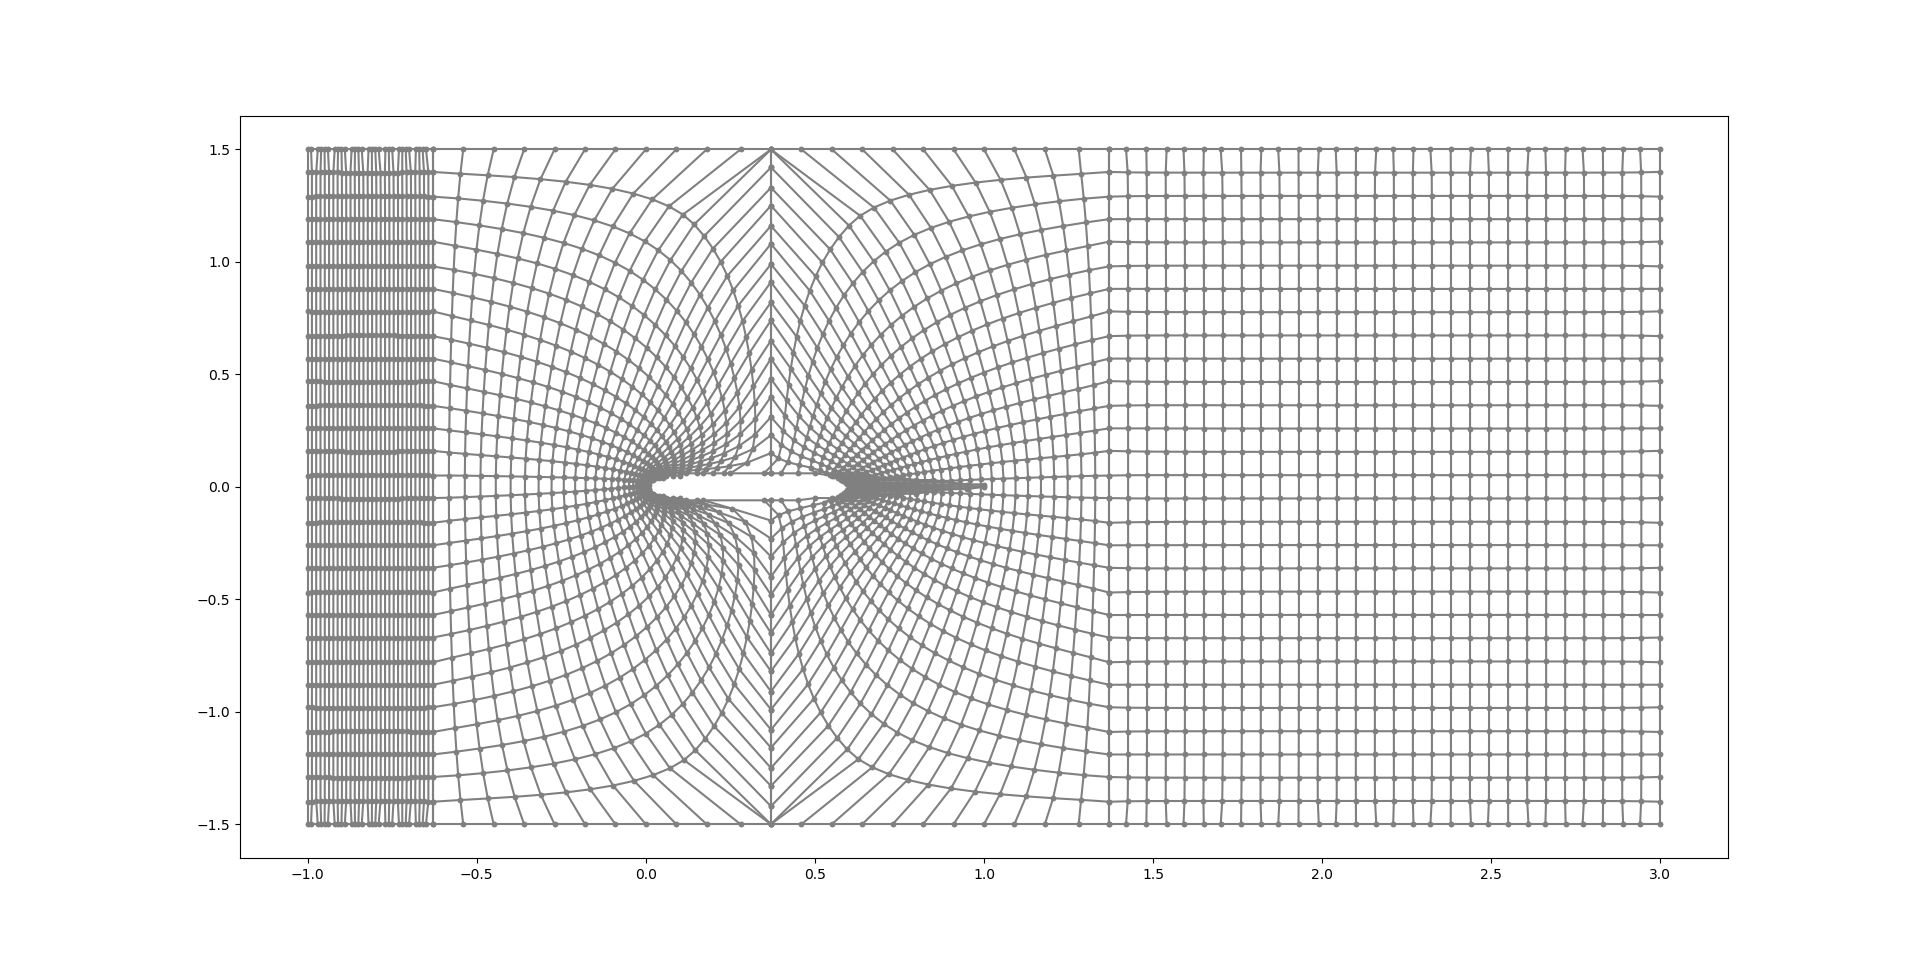
\includegraphics[width=1.0\textwidth]{naca_h1.png}
%	\label{fig:naca_h1} 
%	\caption[caption]{Malha gerada para a curva \textit{naca012 } pela heurística 1 sem refinamento.}
%\end{figure}
%
%\begin{figure}[H]
%	\centering
%	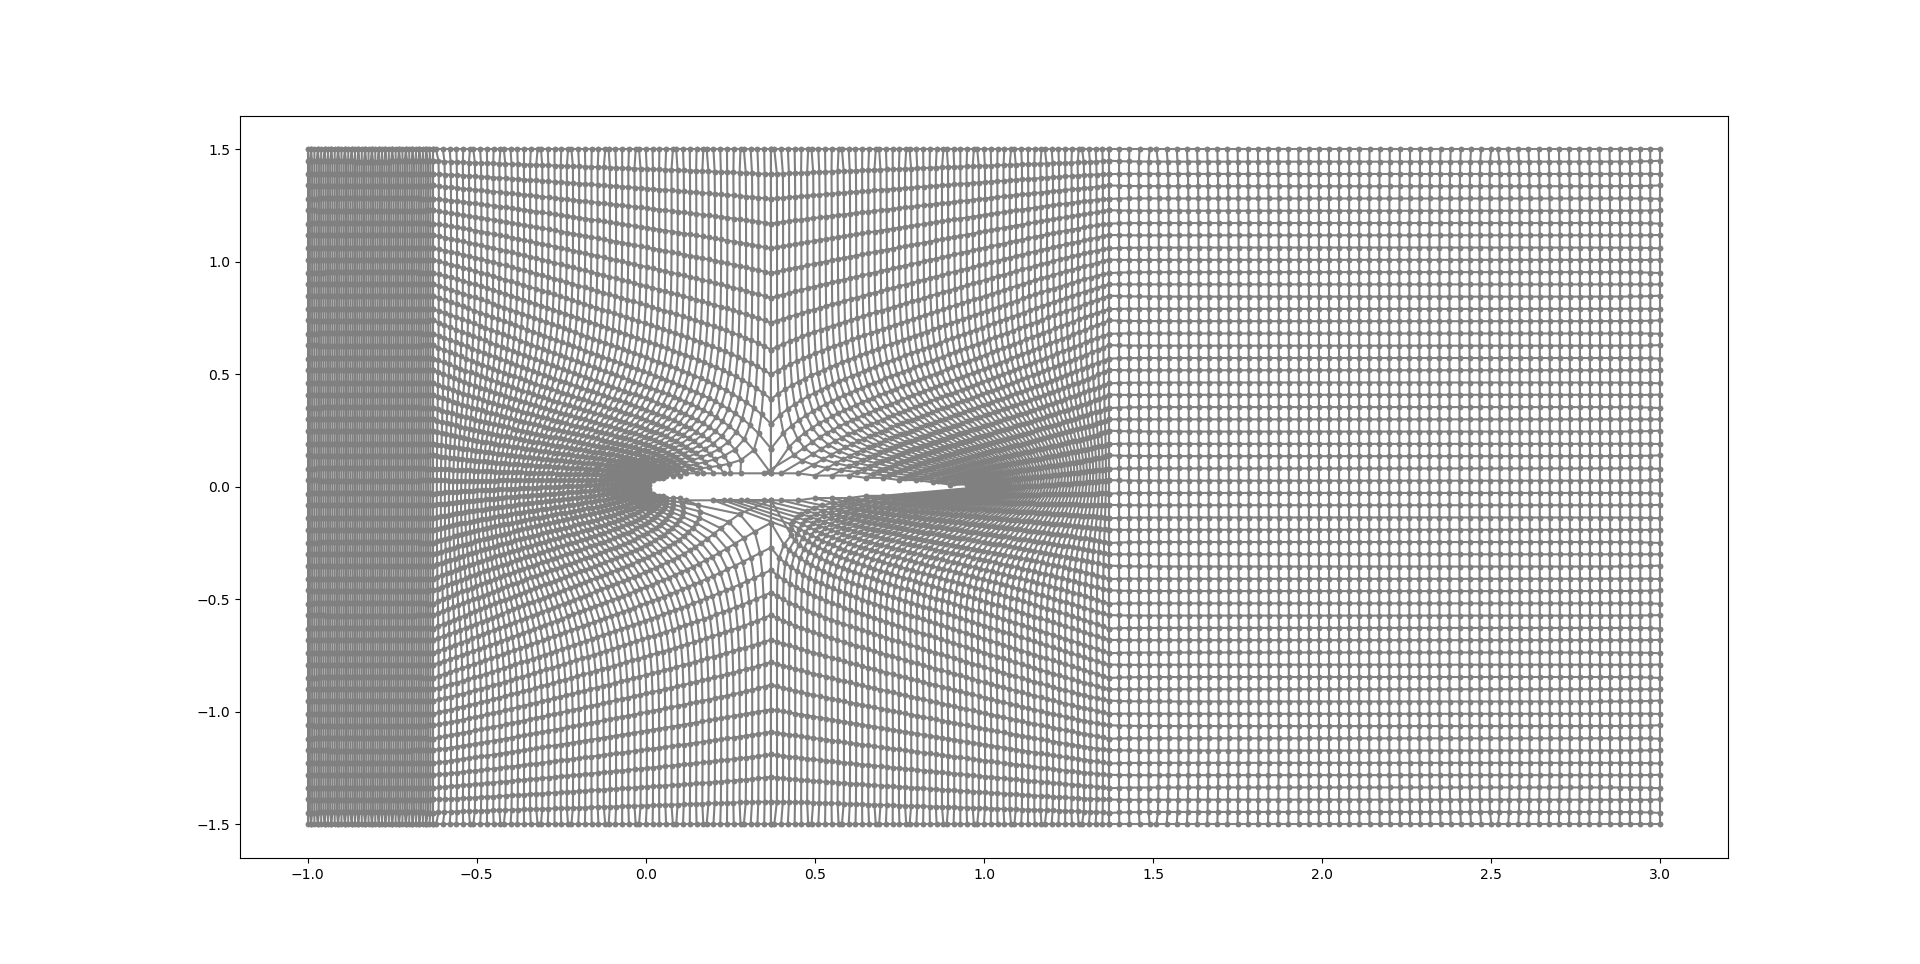
\includegraphics[width=1.0\textwidth]{naca_h2.png}
%	\label{fig:naca_h2} 
%	\caption[caption]{Malha gerada para a curva \textit{naca012 } pela heurística 2 sem refinamento.}
%\end{figure}
%
%
%
%\begin{figure}[H]
%	\centering
%	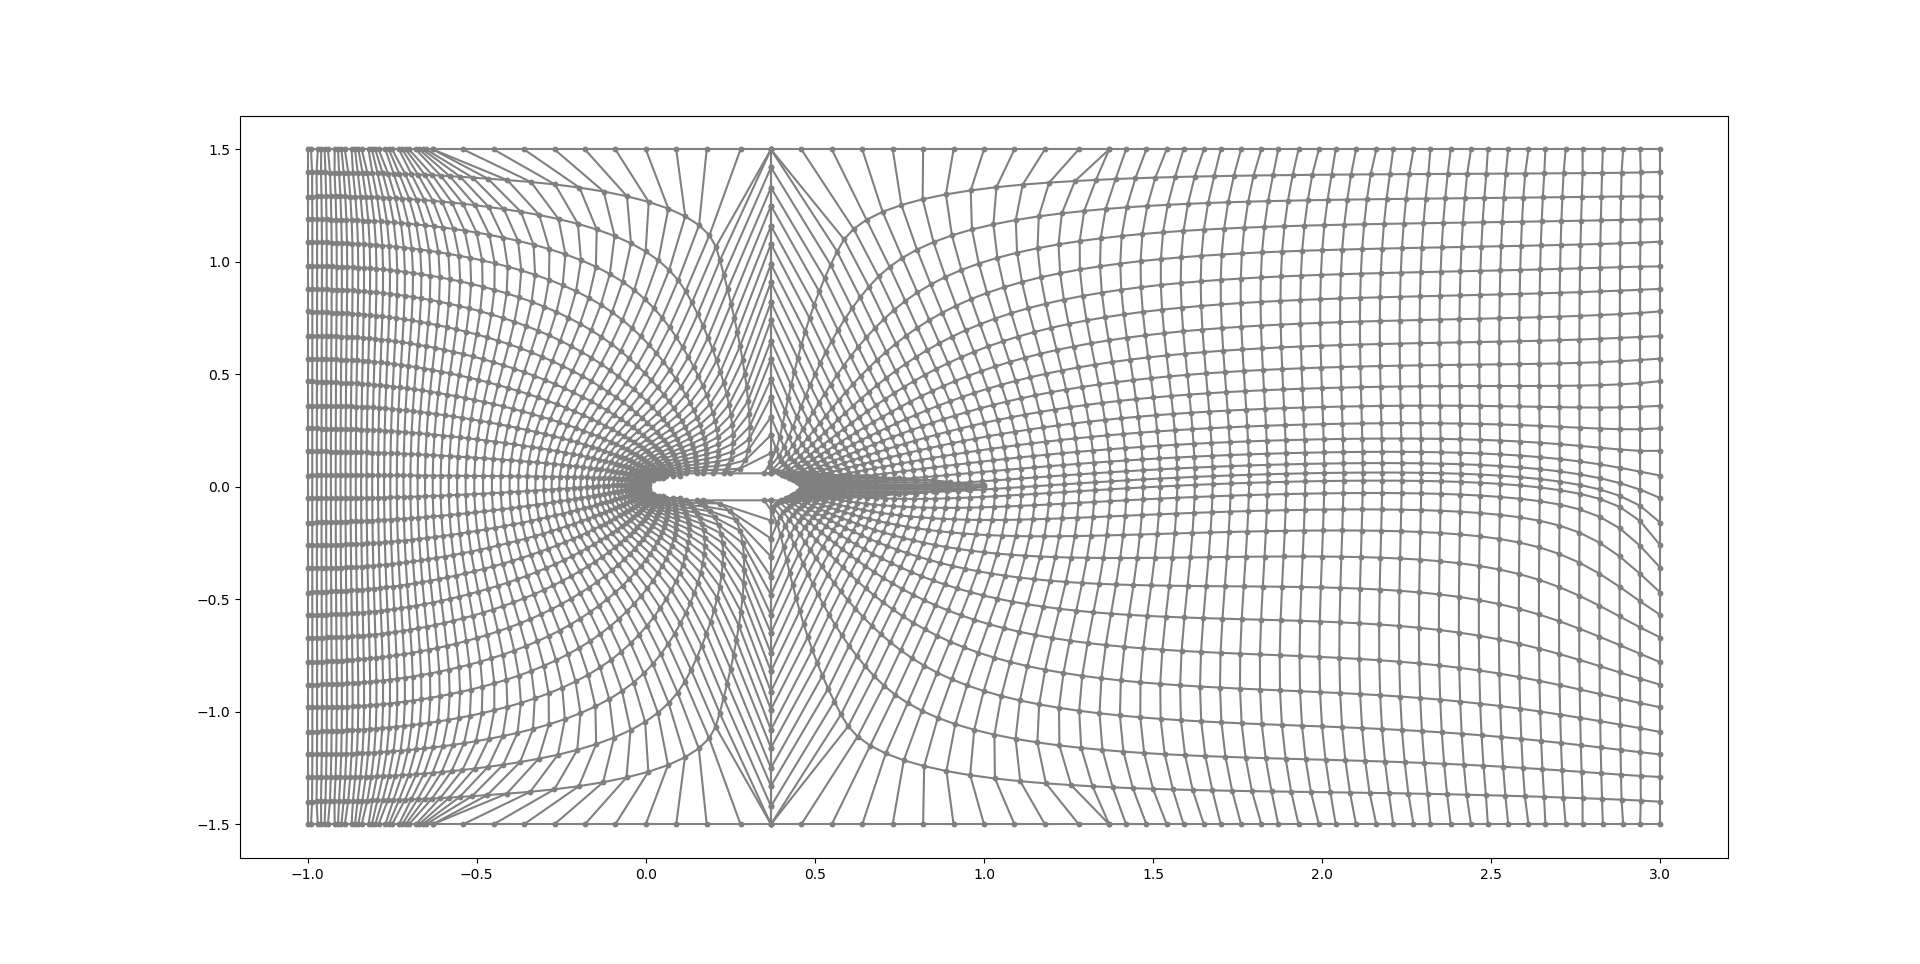
\includegraphics[width=1.0\textwidth]{naca_h1_refined.png}
%	\label{fig:naca_h1_refined} 
%	\caption[caption]{Malha gerada para a curva \textit{naca012 } pela heurística 1 com refinamento.}
%\end{figure}
%
%\begin{figure}[H]
%	\centering
%	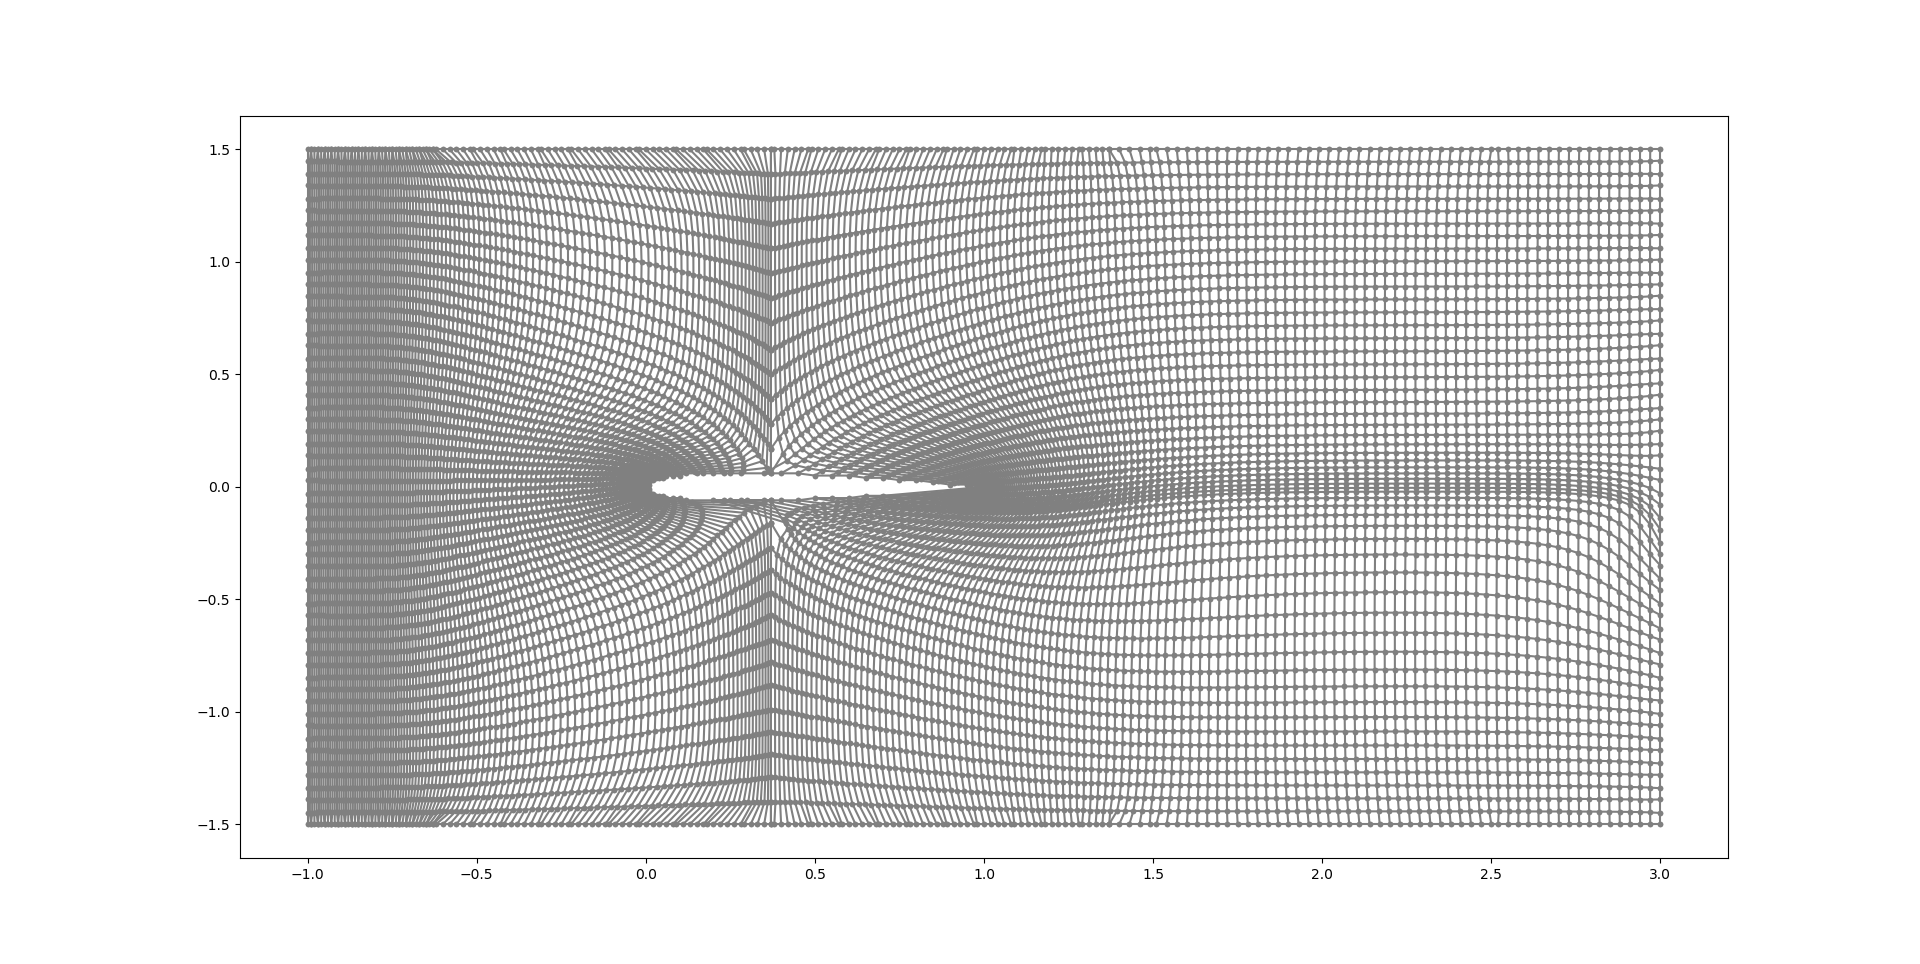
\includegraphics[width=1.0\textwidth]{naca_h2_refined.png}
%	\label{fig:naca_h2_refined} 
%	\caption[caption]{Malha gerada para a curva \textit{naca012 } pela heurística 2 com refinamento.}
%\end{figure}





\end{document}
